\documentclass[12pt,a4paper,figuresright]{book}

\usepackage{amsmath,amssymb}
\usepackage{tabularx,graphicx,url,xcolor,rotating,multicol,epsfig,colortbl}

\setlength{\textheight}{25.2cm}
\setlength{\textwidth}{16.5cm} %\setlength{\textwidth}{18.2cm}
\setlength{\voffset}{-1.6cm}
\setlength{\hoffset}{-0.3cm} %\setlength{\hoffset}{-1.2cm}
\setlength{\evensidemargin}{-0.3cm} 
\setlength{\oddsidemargin}{0.3cm}
\setlength{\parindent}{0cm} 
\setlength{\parskip}{0.3cm}

% -- adding a talk
\newenvironment{talk}[6]% [1] talk title
                         % [2] speaker name, [3] affiliations, [4] email,
                         % [5] coauthors, [6] special session
                         % [7] time slot
                         % [8] talk id, [9] session id or photo
 {%\needspace{6\baselineskip}%
  \vskip 0pt\nopagebreak%
%   \colorbox{gray!20!white}{\makebox[0.99\textwidth][r]{}}\nopagebreak%
%   \ifthenelse{\equal{#9}{photo}}{%
%                     \\\\\colorbox{gray!20!white}{\makebox{\includegraphics[width=3cm]{#8}}}\nopagebreak}{}%
 \vskip 0pt\nopagebreak%
%  \label{#8}%
  \textbf{#1}\vspace{3mm}\\\nopagebreak%
  \textit{#2}\\\nopagebreak%
  #3\\\nopagebreak%
  \url{#4}\vspace{3mm}\\\nopagebreak%
  \ifthenelse{\equal{#5}{}}{}{Coauthor(s): #5\vspace{3mm}\\\nopagebreak}%
  \ifthenelse{\equal{#6}{}}{}{Special session: #6\quad \vspace{3mm}\\\nopagebreak}%
 }
 {\vspace{1cm}\nopagebreak}%

\pagestyle{empty}

% ------------------------------------------------------------------------
% Document begins here
% ------------------------------------------------------------------------
\begin{document}
	
\begin{talk}
  {Sampling multivariate normal distributions under nonlinear constraints}% [1] talk title
  {Hassan MAATOUK}% [2] speaker name
  {EBInnov, School of Industrial Biology, 49 avenue des Genottes,
Cergy-Pontoise, CS 90009, 95895, France}% [3] affiliations
  {h.maatouk@hubebi.com}% [4] email
  {Didier RULLI\`ERE and Xavier BAY}% [5] coauthors
  {}% [6] special session. Leave this field empty for contributed talks. 
				% Insert the title of the special session if you were invited to give a talk in a special session.
			

Generating truncated multivariate normal distributions is widely used in Bayesian statistics [1],  
and is applied in various fields, including ecology, economics, physics, computer science, biology, geosciences, and machine learning.
In this paper, we propose an efficient approach for generating truncated Gaussian vectors subject to both linear and nonlinear constraints.
The main idea is based on absorbing a \textit{smooth relaxation} of the constraints into the likelihood and employing elliptical slice sampling (ESS) [2]. 
For example, in Figure~\ref{fig:tmvn} below, we generate a zero-mean bivariate Gaussian vector restricted to both linear and quadratic constraints (left panel), and to nonlinear constraints (right panel). 
The proposed algorithm outperforms the Hamiltonian Monte Carlo (HMC) approach developed in [3] and implemented in the \texttt{R} package \textit{tmg}. In many cases, the untruncated Gaussian vector exhibits a special structure in the covariance matrix that can enhance the runtime of the proposed algorithm.
The flexibility and performance of the proposed approach have been demonstrated through both synthetic and real data studies in the context of shape-restricted function estimation.


\begin{figure}[ht]
\centering
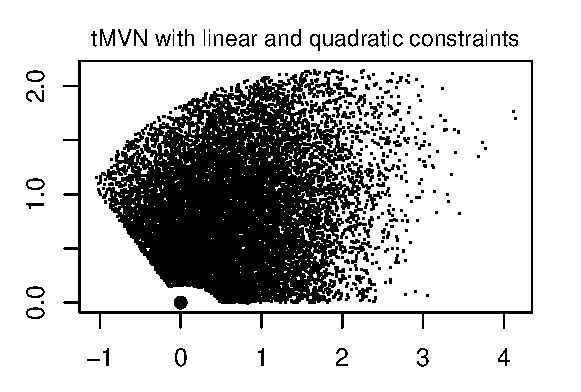
\includegraphics[scale=0.76]{tmvn_linear_quadratic_constr.eps}
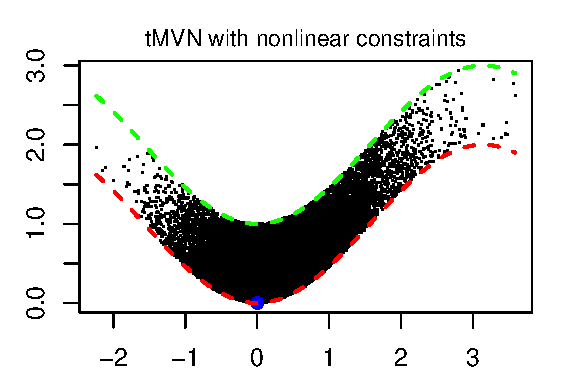
\includegraphics[scale=0.76]{tmvn_nonlinear_constr.eps}
\caption{Sampling 15,000 McMC samples from a bivariate Gaussian vector subject to linear and quadratic constraints (left panel), and to nonlinear constraints (right panel).}
\label{fig:tmvn}
\end{figure}





%\medskip
\section*{References}
\begin{enumerate}
	\item[{[1]}] Maatouk, Hassan \& Xavier Bay (2017). {\it Gaussian process emulators for computer experiments with inequality constraints}. Mathematical Geosciences 49(5):557-582.
	\item[{[2]}] Murray, Iain \& Ryan Prescott Adams \&  David J.C. MacKay (2010). {\it Elliptical slice sampling}. In: Proceedings of the thirteenth international conference on artificial intelligence and statistics, JMLR Workshop and Conference Proceedings, pp 541-548.
	\item[{[3]}] Pakman, Ari \& Liam Paninski (2014). {\it Exact Hamiltonian Monte Carlo for truncated multivariate Gaussians}. Journal of Computational and Graphical Statistics 23(2):518-542.
\end{enumerate}

\end{talk}

\end{document}

